\PassOptionsToPackage{dvipsnames}{xcolor}
\documentclass[
  20pt,
  a0paper,
  portrait,
  margin=0mm,
  innermargin=15mm,
  blockverticalspace=0mm,
  colspace=0mm,
  subcolspace=0mm
]{tikzposter}

% setting page parameters of the poster
\geometry{paperwidth=33in,paperheight=46.7in}

% for includegraphics command
\usepackage{graphicx}

\usepackage{amsmath, amssymb}

% for reduced spacing in references
\usepackage{setspace}

% defining own color in HTML (hex) scheme
\definecolor{mygreen}{HTML}{666633}

% multiple affiliations
\usepackage{authblk}
% setting font and color of authors block
\renewcommand\Authfont{\LARGE \color{white!80!orange}}
% setting font and color of affiliation block
\renewcommand\Affilfont{\Large\color{white!70!mygreen}}

% modern font package
\renewcommand*{\familydefault}{\sfdefault}% Let's have a sans serif font

\usepackage{tikz}
\usetikzlibrary{shapes.geometric, arrows, positioning, decorations.markings}
\usetikzlibrary{fit}
\usepackage{microtype}
\usepackage{framed}
\usetikzlibrary{decorations.pathmorphing,calc,backgrounds}

\newcommand{\mf}{\mathbf}
\newcommand{\lb}{\left(}
\newcommand{\rb}{\right)}

\newcommand{\bbG}{\mathbb{G}}
\newcommand{\bbI}{\mathbb{I}}

\newcommand{\vpravo}{\hspace{1.5cm}}
\newcommand{\vverh}{\vspace*{-0.05cm}}
\newcommand{\vniz}{\vspace{0.05cm}}
% for references:
\newcommand{\hormove}{\par\hangindent 10mm}

\makeatletter
\def\TP@titlegraphictotitledistance{1cm}
\settitle{\centering \color{titlefgcolor} \vbox{\@titlegraphic \\ [\TP@titlegraphictotitledistance] \bfseries \fontsize{1.75cm}{1.3cm} \selectfont \@title \par} \vspace*{1em} {\fontsize{1.4cm}{1cm}\selectfont \@author \par}} 
\makeatother

\title{\parbox{\linewidth}{ \centering First spectral moments of collision-induced rototranslational absorption band of CO$\hspace*{-0.2cm}_2 \hspace{0.2cm}$-Ar pair:} \\
Classical theory with the use of \textit{ab initio} calculated anisotropic interactions}

\author[1, 3]{\underline{Daniil N. Chistikov}}
\author[1]{\underline{Artem A. Finenko}} 
\author[2]{Yulia N. Kalugina}
\author[1, 3]{Sergei E. Lokshtanov}
\author[1]{Sergey V. Petrov}
\author[3]{Andrey A. Vigasin}

\affil[1]{Department of Chemistry, Lomonosov Moscow State University, Leninskie Gory 1-3, Moscow, 119991, Russia}
\affil[2]{Department of Optics and Spectroscopy, Tomsk State University, Lenin av. 36, Tomsk, 634050, Russia}
\affil[3]{Obukhov Institute of Atmospheric Physics Rus.\,Acad.\,Sc., Pyzhevsky per. 3, Moscow, 119017, Russia}

\usetheme{Simple}

\usetitlestyle[width = \linewidth, roundedcorners=5, linewidth=2pt,titletoblockverticalspace=0mm]{Default}
\usebackgroundstyle{Empty}

% this is size of text for References block
\newcommand{\SIZEOFTEXTREFERENCES}{\small}
% this regulates the size of text
\newcommand{\SIZEOFTEXT}{\normalsize}
% this regulates the size of formulae
\newcommand{\SIZEOFFORMULAE}{\fontsize{20}{16}}

\begin{document}

\maketitle

\begin{columns}
\column{0.4}
\block[titleoffsety=44cm, bodyoffsety=45.5cm]{Introduction}{
\SIZEOFTEXT
\SIZEOFFORMULAE{
\vpravo Much attention is presently devoted to the study of dipole-forbidden molecular absorption caused by weak intermolecular interaction. This interest is significantly motivated by the need to refine the accuracy of climate models which are being developed for the planetary or exoplanetary atmospheres. Actual knowledge of binary absorption coefficients is still fragmentary (see e.g. [1]) and is thus fairly unsatisfactory in regard of great number of pairs potentially interesting for climate modeling. Experimental observation of the weak pressure-induced absorption is especially difficult in the far-infrared where the most important so-called rototranslational collision-induced absorption (RT CIA) bands are conventionally situated. Direct quantum calculations are still barely feasible for interacting polyatomics, although significant progress is worth mentioning that has been achieved recently in both quantum calculations of the spectral profiles [2,3] and quantum theory of spectral moments [4,5]. Molecular dynamics simulation and classical trajectory approaches are presently the most promising (see e.g. [6,7]) in terms of purely classical methods. The use of the formerly popular semi-empirical methods is getting more and more senseless nowadays as far as unprecedented computational facility and advancement in quantum chemical methods become available. \par 
\vpravo Present paper aims at theoretical examination of the first spectral moments in rototranslational CIA band of the prototype CO$_2-$Ar system. Our approach relies on the use of anisotropic potential energy and induced dipole surfaces obtained by virtue of sophisticated \textit{ab initio} calculations. The knowledge of these surfaces permits direct classical calculation of the first spectral moments without address to any adjustable parameters. Our ultimate goal consists of development of such a rigorous classical formalism that could permit consideration of CIA in any arbitrary pair formed by typical atmospheric molecules. 

\begin{tikzfigure}
		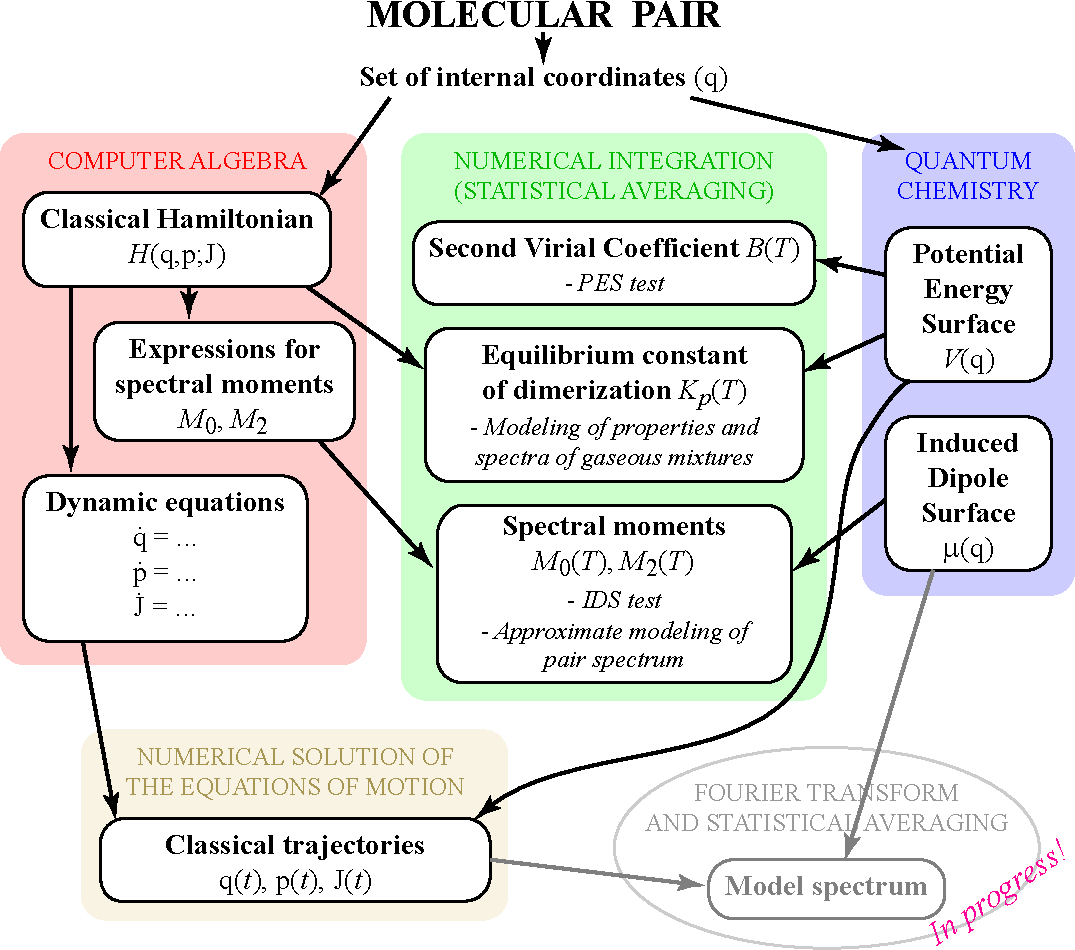
\includegraphics[width=1.0\linewidth]{../pictures/Scheme_1-crop.pdf}
\begin{center}
		Figure 1: Schematic representation of the elements of our approach 
\end{center}
\end{tikzfigure}
}}
\block[titleoffsety=2cm, bodyoffsety=3cm]{General outline of the spectral moment theory}{
\SIZEOFTEXT
\SIZEOFFORMULAE{
\vpravo Spectral moments are integral values, which are widely used to characterise CIA spectra. The use of these values is justified by the possiblity to represent them either in terms of integrals over experimentally measurable spectral profiles or in terms of Boltzmann weighted functions of induced dipole. Thus the knowledge of complete potential energy (PES) and induced dipole (IDS) surfaces can help both verification of \textit{ab initio} obtained data and characterization of interaction-induced absorption. \par

\vpravo Two systems of coordinates are conventionally employed in theoretical consideration of collisional dynamics among polyatomic molecules. These are so-called laboratory- and body-fixed frames. Salient feature of our approach consists of development and subsequent use of rigorous classical Hamiltonian in the body-fixed frame. All kinetic energy terms that are responsible for Coriolis interaction are kept in derived Hamiltonian. In its general form the latter can be represented as  
\vverh
\begin{gather}
		H = \frac{1}{2} \mf{p}^\top \bbG_{11} \lb \mf{q} \rb \mf{p} + \mf{p}^\top \bbG_{12} \lb \mf{q} \rb \, \mf{J} + \frac{1}{2} \mf{J}^\top \bbG_{22} \lb \mf{q} \rb \, \mf{J} + U(\mf{q}), \label{eq:hamiltonian}
\end{gather}
where $\mf{q}$, $\mf{p}$ denote the generalized coordinates and conjugated momenta, $\mf{J}$ denotes the vector of total angular momentum. For any molecular pair under consideration the exact expressions for elements of matrices $\bbG$ are obtained by means of computer algebra. The binary absorption coefficient, $\alpha \lb \nu \rb$, is related to the spectral function, $g \lb \nu \rb$, according to [8] 
\vverh
\begin{gather}
		\alpha \lb \nu \rb = \frac{\lb 2 \pi \rb^3 N_a^2}{3 \hbar} \rho_1 \rho_2 \, \nu \left[ 1 - \exp \lb - \frac{h c \nu}{k T} \rb \right] g \lb \nu \rb \notag
\end{gather}

The $n$-th spectral moment of the spectral function, $g(\nu)$, is defined by 
\vverh
\begin{gather}
		M_n = \int\limits_{-\infty}^{\infty} \nu^n g(\nu) d \nu \label{eq:gen_moment} 
\end{gather}

In the classical limit the following expressions are used to calculate spectral moments [8]:
\vspace*{-0.6cm}
\begin{gather}
\begin{aligned}
		M_{2n} = V \lb 2 \pi c \rb^{-n} & \frac{1}{4 \pi \varepsilon_0} \Big\langle \Big{|} \frac{d^n}{dt^n} \boldsymbol{\mu}(t) \Big{|}^2 \Big\rangle \Bigg{|}_{t = 0} \\
M_{2n + 1} &= 0
\end{aligned}
\label{eq:classical_moment}
\end{gather}
where $\boldsymbol{\mu}$ denotes the vector of dipole moment and angular brackets denote averaging over the complete phase space. Specifically, classical expressions for lowest-order zeroth and second spectral moments can be written as
\begin{gather}
		M_0 = \displaystyle \frac{\int \boldsymbol{\mu}^2 \exp \lb -H \lb \mf{q}, \mf{p}, \mf{J} \rb / k T \rb d \mf{q} \, d \mf{p}}{\int \exp \lb - H \lb \mf{q}, \mf{p}, \mf{J} \rb / k T \rb d \mf{q} \, d \mf{p}}, \quad M_2 = \displaystyle \frac{\int \boldsymbol{\dot{\mu}}^2 \exp \lb -H \lb \mf{q}, \mf{p}, \mf{J} \rb / k T \rb d \mf{q} \, d \mf{p}}{\int \exp \lb - H \lb \mf{q}, \mf{p}, \mf{J} \rb / k T \rb d \mf{q} \, d \mf{p}}. \label{eq:m0_and_m2} 
\end{gather}

The expression for the second moment includes time derivative of the dipole which can be calculated from the Poisson bracket using classical Hamiltonian
\begin{gather}
		\frac{d \boldsymbol{\mu}}{dt} = \left[ \boldsymbol{\mu}, H \right] = \sum_i \left\{ \frac{\partial \boldsymbol{\mu}}{\partial q_j} \frac{\partial H}{\partial p_j} 
		- \frac{\partial \boldsymbol{\mu}}{\partial p_j} \frac{\partial H}{\partial q_j} \right\}. \label{eq:poisson} 
\end{gather}
Obviously, the IDS is determined by spatial position of interacting moieties and does not depend on their velocities (conjugated momenta). That is why we are interested only in derivatives of the Hamiltonian over momenta which can be calculated numerically at any point of the phase space using matrix formalism. \par 
Assuming the Hamiltonian is written in the body-fixed frame (BF), the squared time derivative of the dipole in laboratory frame (LF) can be written as:
\begin{gather}
		\lb \boldsymbol{\dot{\mu}}^{LF} \rb^2 =  \lb \boldsymbol{\dot{\mu}}^{BF} \rb^2 + 2 \boldsymbol{\mu}^{BF} \left( \frac{\partial H}{\partial \mf{J}} \times \boldsymbol{\mu}^{BF} \right) + \lb \boldsymbol{\mu}^{BF} \rb^\top \bbI^J \boldsymbol{\mu}^{BF}, \label{eq:dipole2} 
\end{gather}
where elements of matrix $\bbI^J$ are defined as 
\begin{gather}
\bbI^J_{ij} = \sum_{k} \lb \frac{\partial H}{\partial J_k} \rb^2 \delta_{ij} - \lb \frac{\partial H}{\partial J_i} \rb \lb  \frac{\partial H}{\partial J_j} \rb \label{eq:I_matrix}
\end{gather}

}}
\column{0.6}
\block[titleoffsety=44cm, bodyoffsety=45.5cm]{Spectral moments of CO$_2-$Ar rototranslational band}{
\SIZEOFTEXT
\SIZEOFFORMULAE{
\vpravo In the present paper we have chosen CO$_2-$Ar as an example of relatively simple atom-linear molecule system possessing an appreciable anisotropy of interaction (Fig. 1). Assuming rigid CO$_2$, position of interacting CO$_2$ and Ar species in the body-fixed frame can be represented using two internal coordinates. Potential energy surface (PES) as a function of these coordinates was calculated in our work using CCSD(T) method with \textit{aug-cc-pvQZ} basis set supplemented with mid-bond functions. \par 
\vpravo The dipole (IDS) was calculated using either CCSD(T) level of \textit{ab initio} theory with \textit{aug-cc-pvTZ} basis set or using the so-called long-range approximation that assumes IDS having been represented as a series over CO$_2$ multipole moments up to hexadecapole. The $z$-components of \textit{ab initio} and long-range dipoles as functions of $r$ for two configurations are shown on Fig.\,2. \par
\vpravo Our calculated $T$-dependences for the zeroth and second spectral moments are shown in Figs. 3, 4, respectively. The symbols in these figures relate to the data obtained from available [8, 9] experimental binary absorption coefficients $\alpha(\nu)$ using the integrals:
\vverh
\begin{gather}
		M_0 = \frac{1}{\rho_1 \rho_2} \int\limits_{0}^{\infty} \alpha(\nu) \coth \lb - \frac{h c \nu}{2 k T} \rb \frac{d \nu}{\nu}, \quad M_2 \approx \frac{1}{\rho_1 \rho_2} \int\limits_{0}^{\infty} \alpha(\nu) d \nu. \label{eq:m2_spectra}
\end{gather}

\begin{minipage}{0.5\linewidth}
%\hbox to \hsize{%
\begin{tikzfigure}
\vspace*{-1cm}
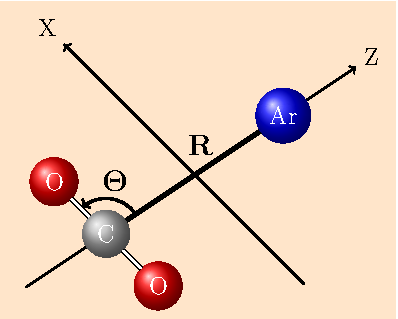
\includegraphics[width=0.8\linewidth]{../pictures/coordsys/pp/coordsys-crop.pdf}
\label{fig:coordsys}
\end{tikzfigure} 
\end{minipage}
\begin{minipage}{0.5\linewidth}
\begin{tikzfigure}
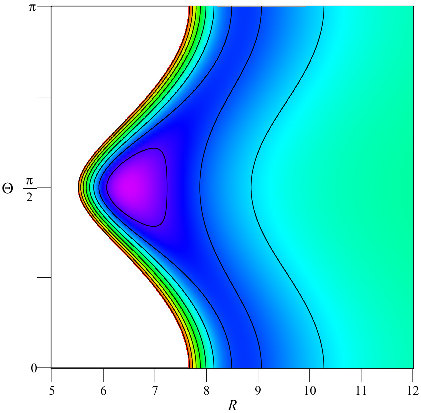
\includegraphics[width=0.75\linewidth]{../pictures/potential/potential_dpi.pdf}
\label{fig:potential}
\end{tikzfigure}
\end{minipage}
\vspace*{-1cm}
\begin{gather}
H = \frac{1}{2 \mu_2} p_R^2 + \lb \frac{1}{2 \mu_2 R^2} + \frac{1}{2 \mu_1 l^2} \rb p_\theta^2 - \frac{1}{\mu_2 R^2} p_\theta J_y + \frac{1}{2 \mu_2 R^2} J_y^2 + \frac{1}{2 \mu_2 R^2} J_x^2 + \frac{1}{2 \sin^2 \theta} \lb \frac{\cos^2 \theta}{\mu_2 R^2} + \frac{1}{\mu_1 l^2} \rb J_z^2 
+ \frac{\cot \theta}{\mu_2 R^2} J_x J_z + U(R, \theta), \notag \\
\mu_1 = m_{\textup{O}} / 2, \mu_2 = m_{\textup{Ar}} m_{\textup{CO}_2} / (m_{\textup{Ar}} + m_{\textup{CO}_2}) \notag
\end{gather}
\begin{center}
Figure 2: Coordinate system, potential energy surface (PES) and classical Hamiltonian for CO$_2 \hspace{0.1cm}$-Ar
\end{center}

\vspace{1cm}
\begin{minipage}{0.5\linewidth}
\begin{tikzfigure}
		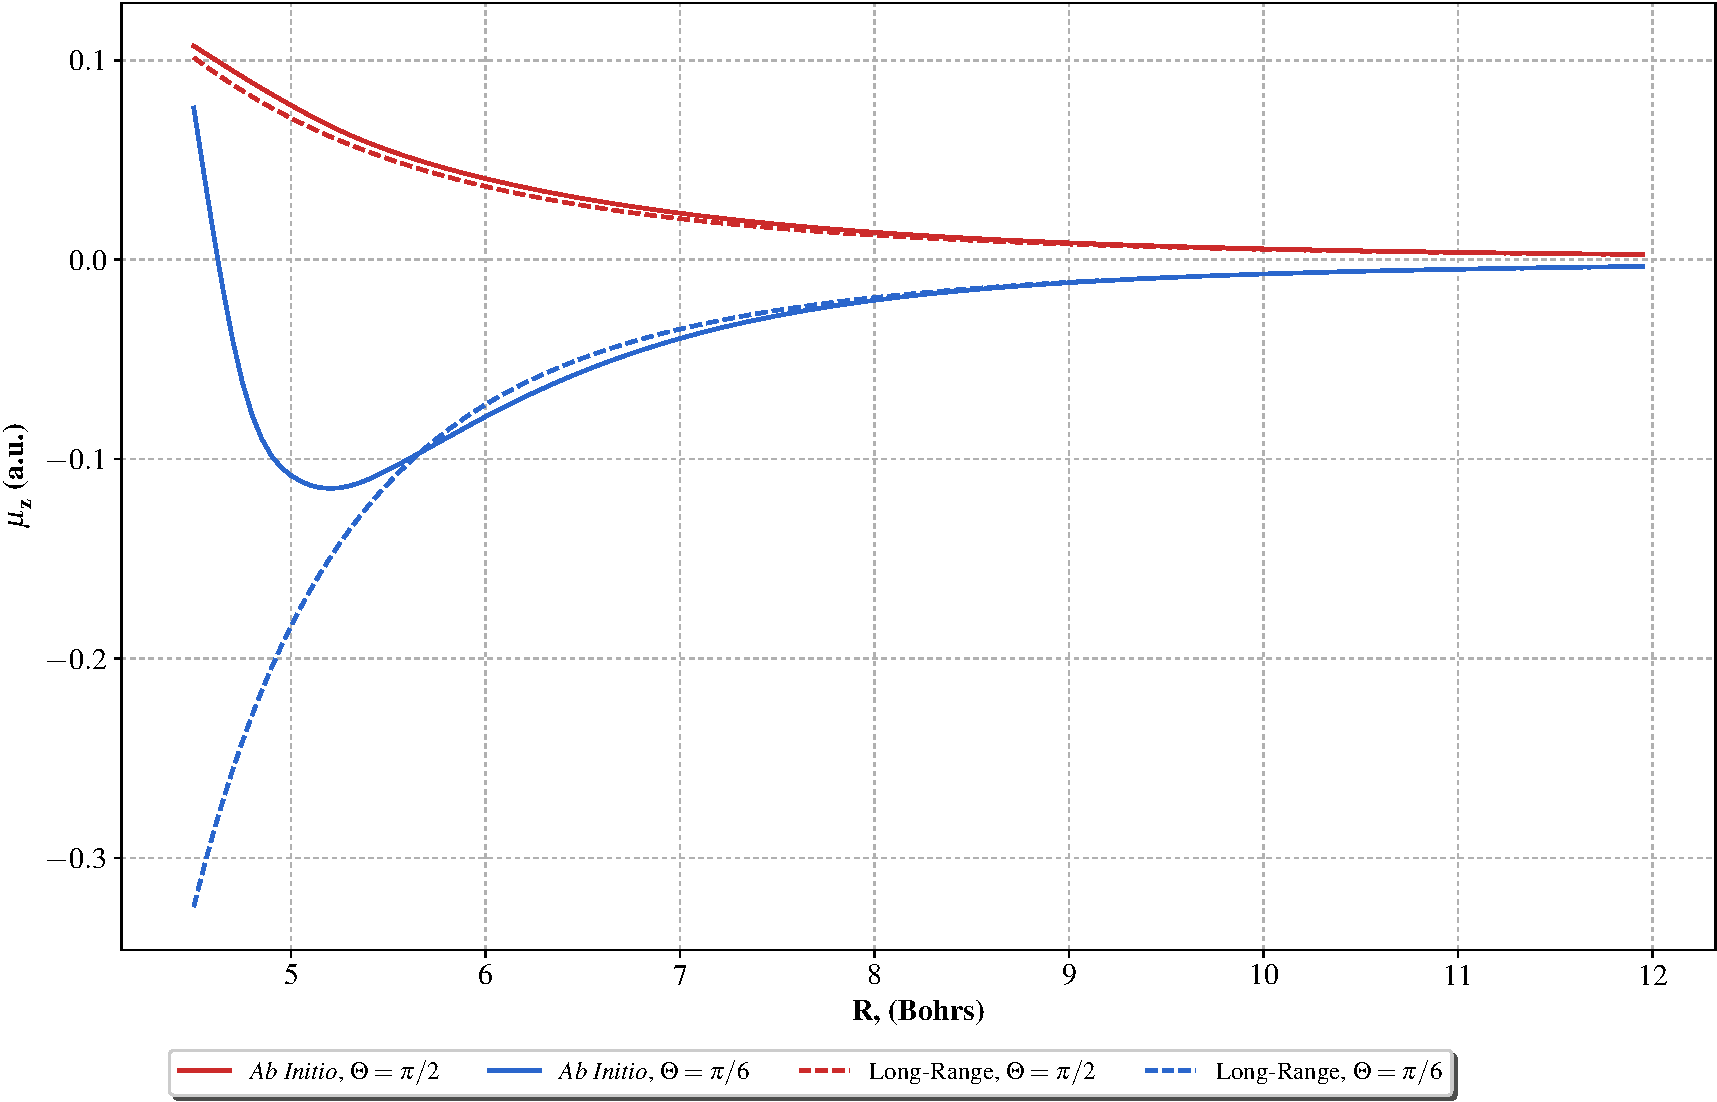
\includegraphics[height=17cm,width=0.95\linewidth]{../pictures/dipole_pictures/last-crop.pdf}
\end{tikzfigure}
\begin{center}
\vspace*{-0.5cm}
Figure 3: Z-components of the dipole moment \label{fig:dipole}
\end{center}
\end{minipage}
\begin{minipage}{0.5\linewidth}
\begin{tikzfigure}
		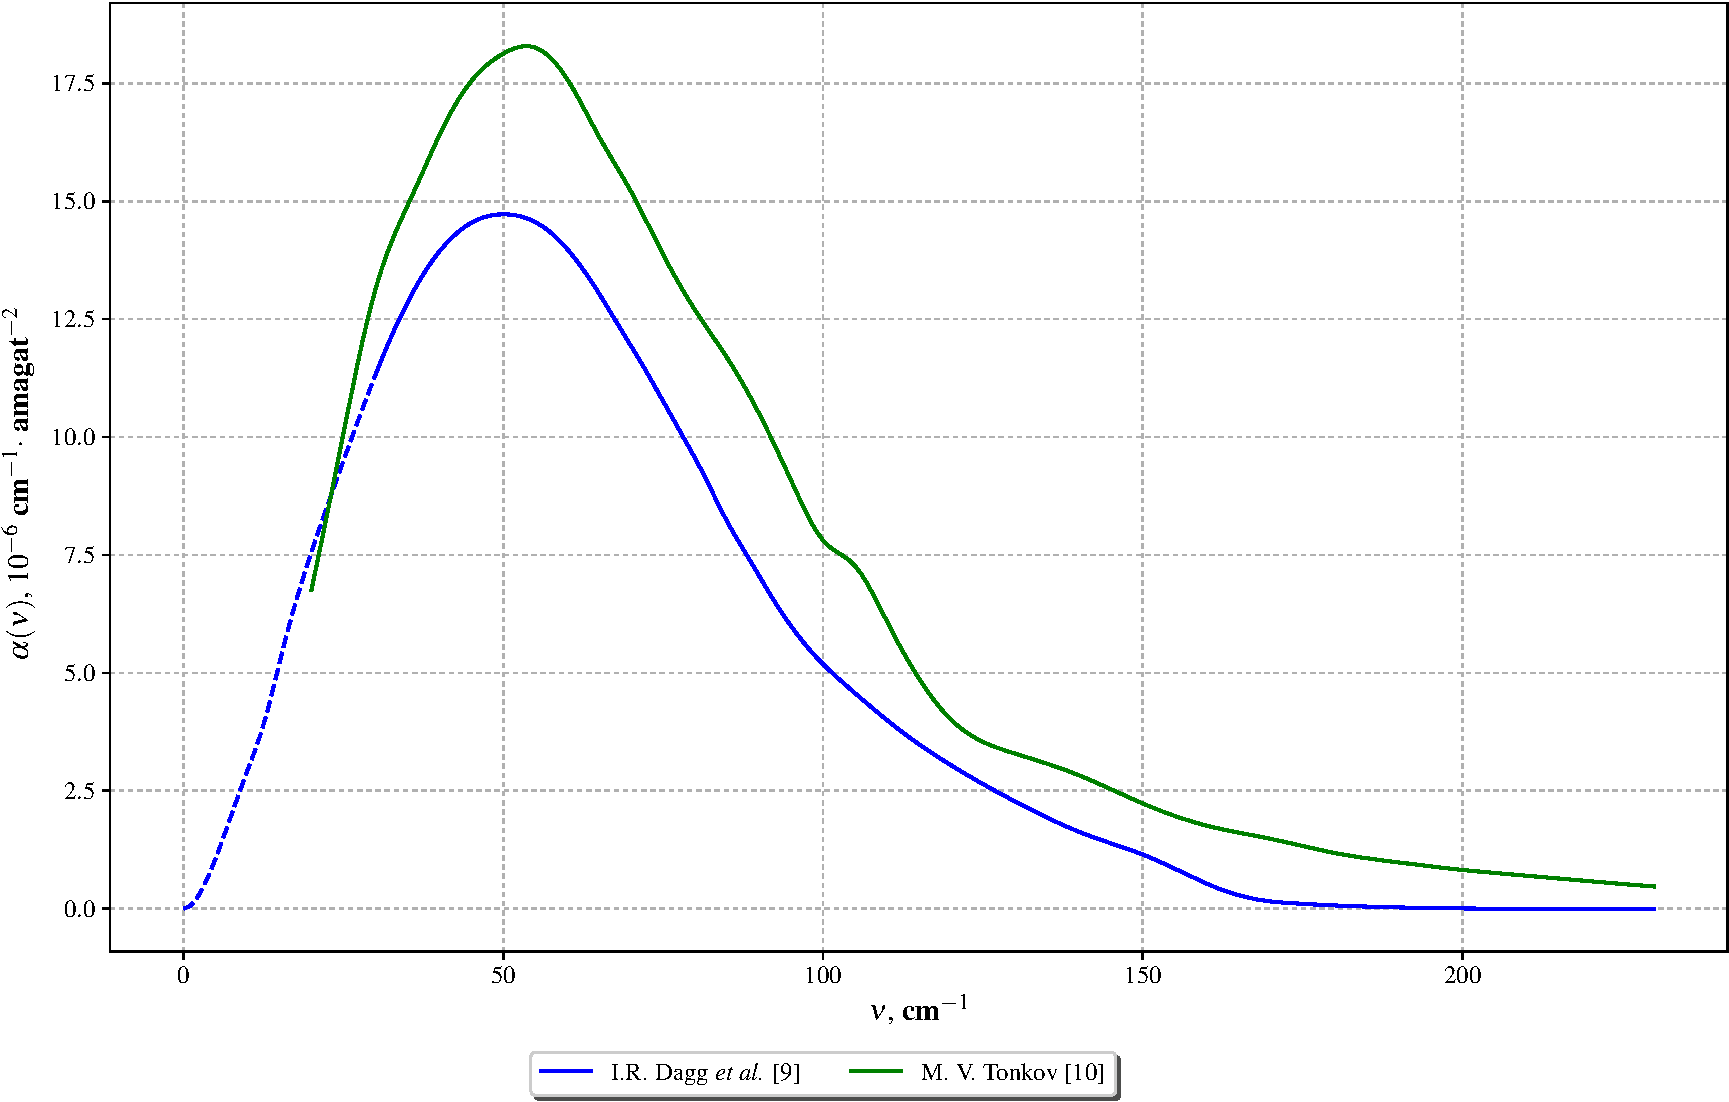
\includegraphics[height=17cm,width=\linewidth]{../pictures/spec_picture/spec_picture-crop.pdf}
\end{tikzfigure}
		\vspace*{-1cm}
		\begin{center}
				Figure 4. Experimental absorption spectra of CO$_2-$Ar 
		\end{center}
\end{minipage}

\vspace{1cm}

\begin{tikzfigure}
\hbox to \hsize{%	
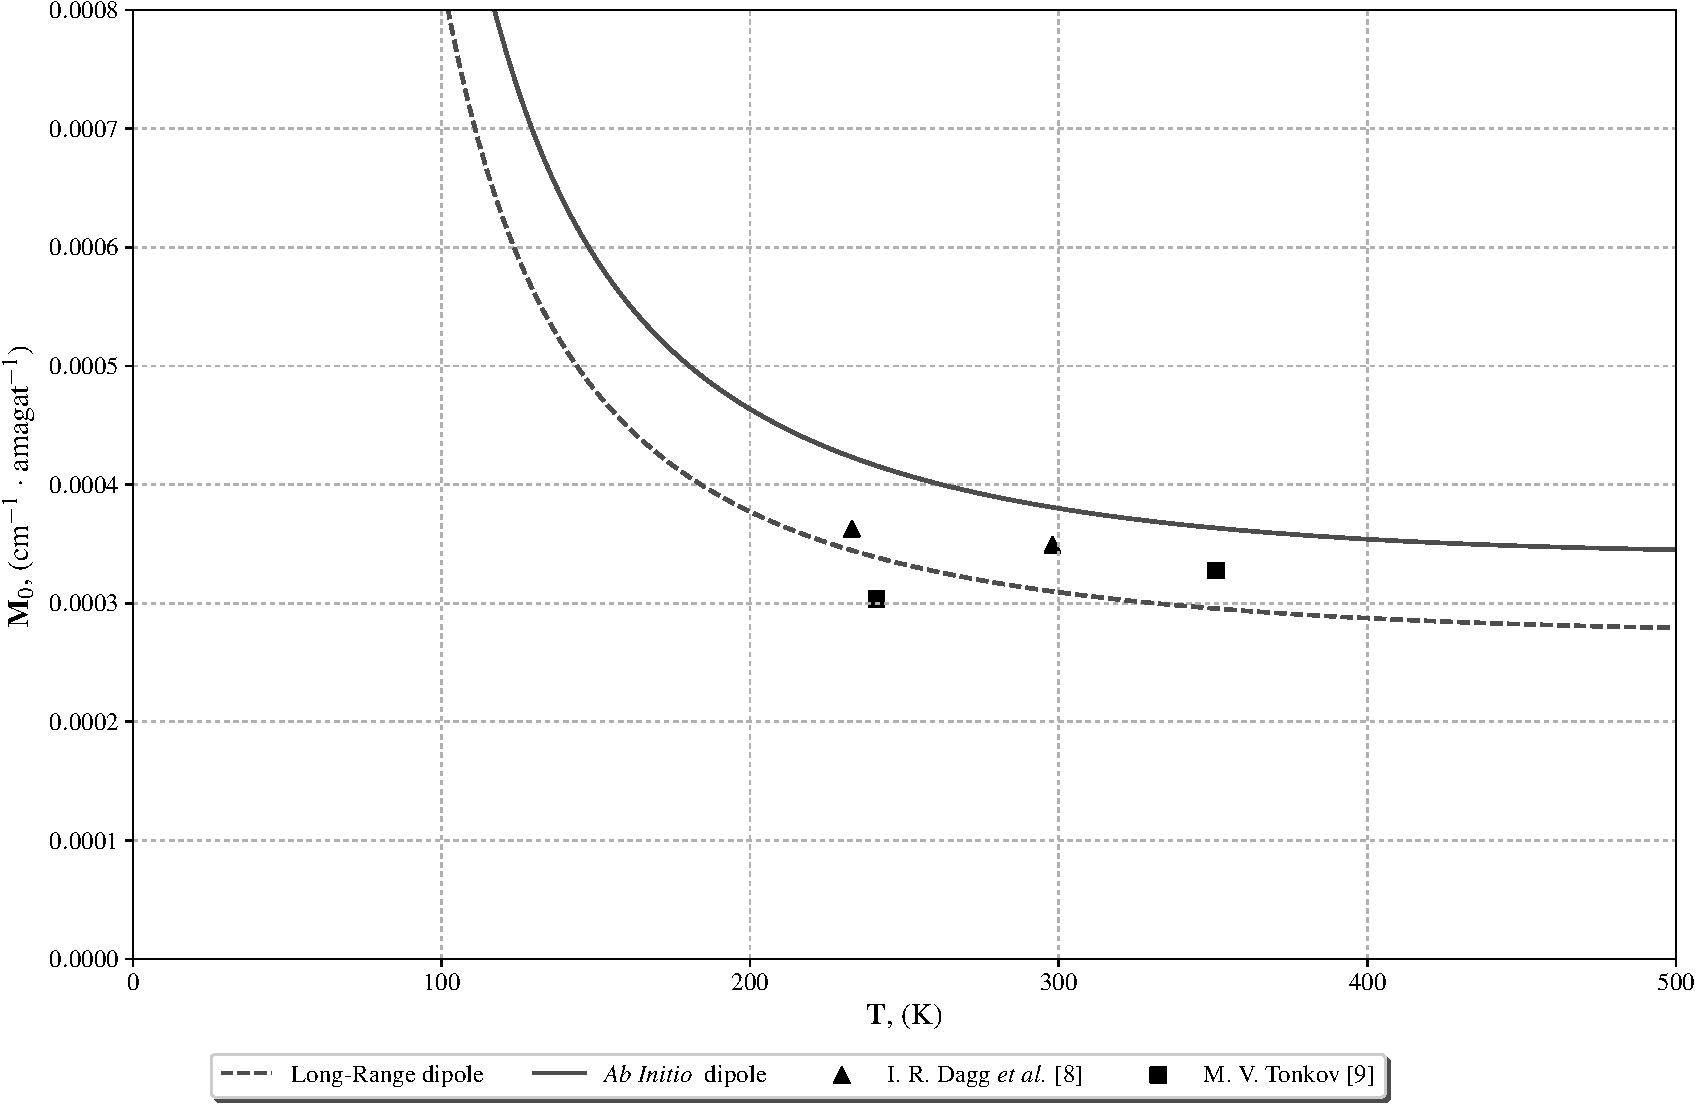
\includegraphics[height=17cm, width=0.49\linewidth]{../pictures/moments_pictures/moment0/last0-crop.pdf}%
\hss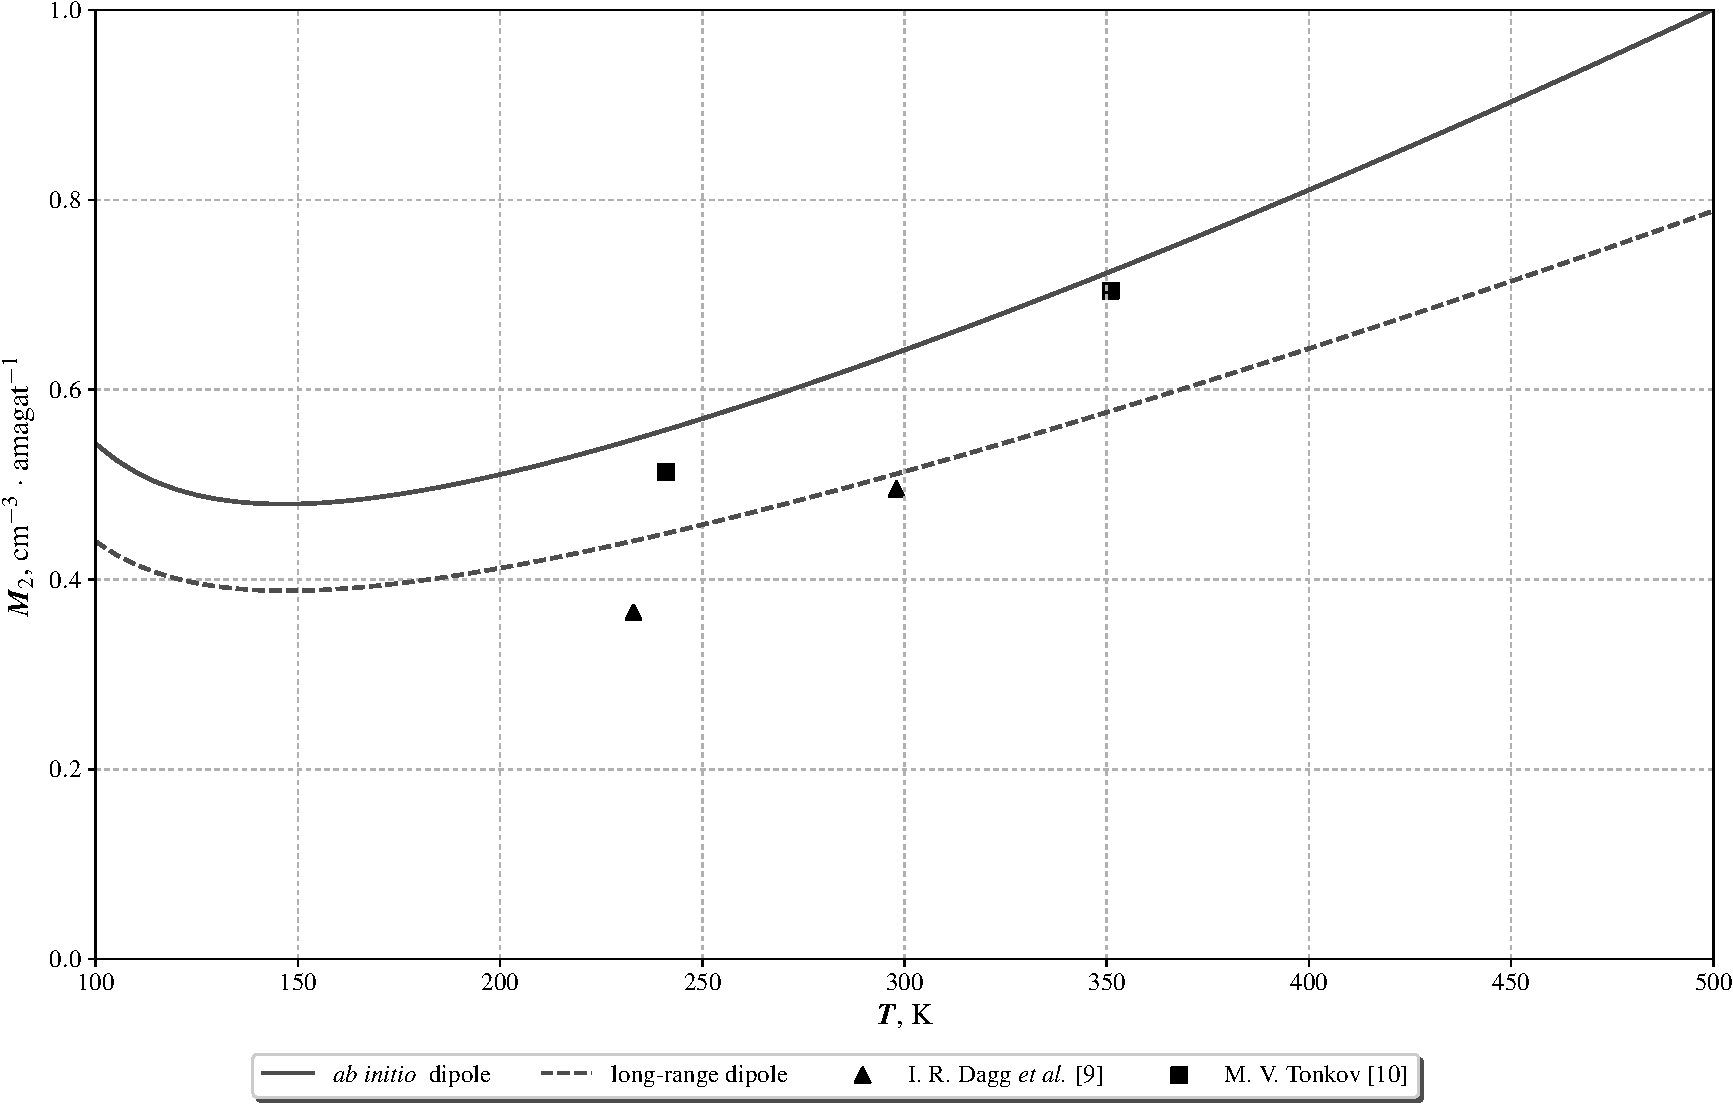
\includegraphics[height=17cm, width=0.49\linewidth]{../pictures/moments_pictures/moment2/last2-crop.pdf}}
\end{tikzfigure}
\begin{center}
		\vspace*{-1cm}
		Figure 5: Temperature dependences of zeroth and second spectral moments
\end{center}
}}

\block[titleoffsety=1.5cm, bodyoffsety=3cm]{Conclusions}{
\SIZEOFTEXT
\SIZEOFFORMULAE{
\vpravo The results reported in the present paper demonstrate capability of classical methods to characterize collision-induced absorption in the far-infrared spectral range with an accuracy comparable with that experimental. No use of adjustable parameters is required provided potential energy and induced dipole surfaces are obtained as a result of the high-level \textit{ab initio} calculations and no omission is made in kinetic energy terms of the classical Hamiltonian. The results obtained so far encourage us to extend our approach to other molecular pairs the knowledge of the dipole-forbidden absorption in which is in high demand by the planetary atmospheres investigators. 
}}

\block[titleoffsety=1.0cm, bodyoffsety=2.5cm]{References}{
\SIZEOFTEXTREFERENCES
\begin{spacing}{0.1}
% I know the code is horrible.. 
% \! -- negative \thinmuskip 
%
\advance\parskip by 2.0mm
\parindent 0mm
\hangindent 10mm
\hspace*{-0.1cm}\ 1.\ C. Richard, I.\! E. Gordon, L.\! S. Rothman \textit{et al} (2012). New section of the HITRAN database: Collision-induced absorption (CIA). \textit{Journal of Quantitative Spectroscopy and Radiative Transfer}, 113(11), 1276-1285. \hormove 
\ 2.\ T. Karman, A. van der Avoird, G.\! C. Groenenboom (2015). Collision-induced absorption with exchange effects and anisotropic interactions: Theory and application to H$_2$\! - \!H$_2$. \textit{The Journal of chemical physics}, 142(8), 084305. \hormove
\ 3.\ T. Karman, E. Miliordos, K.\! L. Hunt, G.\! C. Groenenboom, A. van der Avoird (2015). Quantum mechanical calculation of the collision-induced absorption spectra of N$_2$\! - \!N$_2$ with anisotropic interactions. \textit{The Journal of chemical physics}, 142(8), 084306. \hormove
\ 4.\ M. Chrysos, A.\! P. Kouzov, N.\! I. Egorova, F. Rachet (2008). Exact Low-Order Classical Moments in Collision-Induced Bands by Linear Rotors: CO$_2$\! - \!CO$_2$. \textit{Physical review letters}, 100(13), 133007. \hormove
\ 5.\ A.\! P. Kouzov, M. Chrysos (2009). Collision-induced absorption by CO$_2$ in the far infrared: Analysis of leading-order moments and interpretation of the experiment. \textit{Physical Review A}, 80(4), 042703. \hormove
\ 6. \!J.\! M. Hartmann, C. Boulet, D. Jacquemart (2011). Molecular dynamics simulations for CO$_2$ spectra. II. The far infrared collision-induced absorption band. \textit{The Journal of chemical physics}, 134(9), 094316. \hormove
\ 7.\ D.\! V. Oparin, N.\! N. Filippov, I.\! M. Grigoriev, A.\! P. Kouzov (2017). Effect of stable and metastable dimers on collision-induced rototranslational spectra: Carbon dioxide-rare gas mixtures. \textit{Journal of Quantitative Spectroscopy and Radiative Transfer}, 196, 87-93.\hormove
\ 8.\ L. Frommhold (2006) \textit{Collision-induced absorption in gases}. Cambridge University Press. \hormove
\ 9.\ I.\! R. Dagg \textit{et al.} (1986), \textit{Canadian Journal of Physics}  64, 1485. \par 
10.\ M.\! V. Tonkov (1995) In: \textit{Collision- and Interaction-Induced Spectroscopy}. Kluwer AP. \\
\hspace*{-5cm}
\begin{flushright}
		\textbf{Partial support from RFBR Grants 15-05-00736 and 15-03-03302 is gratefully acknowledged.}
\end{flushright}
\end{spacing}
}}

\end{columns}

\end{document}


Classical expressions are obtained for the zeroth and the second spectral moments in which anisotropy of intermolecular interaction is explicitly taken into account for the first time. The comparison of our calculated and available experimental data is discussed for both mixed second virial coefficient and spectral moments of the RT CIA band in $CO_2-Ar$ pairs. \par

DRAFT OF THE FIRST PARAGRAPH OF "CALCULATION OF SPECTRAL MOMENTS"
Spectral moments are integral quantity widely used for describing CIA spectral profiles. It is used to verify IDS and predicted CIA spectral profiles and also for semi-empirical estimation of CIA spectra. \par
\vpravo For our further discussion we consider two systems of coordinates for describing the relative motion of the colliding pair. First one, called laboratory frame of reference, is fixed with the center of mass of pair and second one, called body-fixed frame, is connected to the pair itself and rotates along with it. Salient feature of our approach consists of development and subsequent use of a rigorous classical Hamiltonian in the body-fixed frame. All kinetic energy terms that are responsible for Coriolis interaction are kept in developed Hamiltonian. The general form of the Hamiltonian is as follows: 

\block[titleoffsety=1.0cm, bodyoffsety=2.5cm]{References}{
\SIZEOFTEXTREFERENCES
\begin{spacing}{0.1}
% I know the code is horrible.. 
% \! -- negative \thinmuskip 
%
\hormove 1. \!\!C. Richard, I.\! E. Gordon, L.\! S. Rothman \textit{et al} (2012). New section of the HITRAN database: Collision-induced absorption (CIA). \textit{Journal of Quantitative Spectroscopy and Radiative Transfer}, 113(11), 1276-1285. \\ \hormove 
2. \!T. Karman, A. van der Avoird, G.\! C. Groenenboom (2015). Collision-induced absorption with exchange effects and anisotropic interactions: Theory and application to H$_2$\! - \!H$_2$. \textit{The Journal of chemical physics}, 142(8), 084305. \\ \hormove
3. \!T. Karman, E. Miliordos, K.\! L. Hunt, G.\! C. Groenenboom, A. van der Avoird (2015). Quantum mechanical calculation of the collision-induced absorption spectra of N$_2$\! - \!N$_2$ with anisotropic interactions. \textit{The Journal of chemical physics}, 142(8), 084306. \\ \hormove
4. \!M. Chrysos, A.\! P. Kouzov, N.\! I. Egorova, F. Rachet (2008). Exact Low-Order Classical Moments in Collision-Induced Bands by Linear Rotors: CO$_2$\! - \!CO$_2$. \textit{Physical review letters}, 100(13), 133007. \\ \hormove
5. \!A.\! P. Kouzov, M. Chrysos (2009). Collision-induced absorption by CO$_2$ in the far infrared: Analysis of leading-order moments and interpretation of the experiment. \textit{Physical Review A}, 80(4), 042703. \\ \hormove
6. \!J.\! M. Hartmann, C. Boulet, D. Jacquemart (2011). Molecular dynamics simulations for CO$_2$ spectra. II. The far infrared collision-induced absorption band. \textit{The Journal of chemical physics}, 134(9), 094316. \\ \hormove
7. \!D.\! V. Oparin, N.\! N. Filippov, I.\! M. Grigoriev, A.\! P. Kouzov (2017). Effect of stable and metastable dimers on collision-induced rototranslational spectra: Carbon dioxide-rare gas mixtures. \textit{Journal of Quantitative Spectroscopy and Radiative Transfer}, 196, 87-93. \\ \hormove
8. \!L. Frommhold (2006) \textit{Collision-induced absorption in gases}. Cambridge University Press. \\ \hormove
9. \!I.\! R. Dagg \textit{et al.} (1986), \textit{Canadian Journal of Physics}  64, 1485. \\ \hspace*{-0.58cm}
10. \!M.\! V. Tonkov (1995) In: \textit{Collision- and Interaction-Induced Spectroscopy}. Kluwer AP. \\
\hspace*{-5cm}
\begin{flushright}
		\textbf{Partial support from RFBR Grants 15-05-00736 and 15-03-03302 is gratefully acknowledged.}
\end{flushright}
\end{spacing}


